\chapter{TOOLS AND TECHNIQUES}

\section{Overview}
The software tools and development platforms utilized for the planned final year project's design, implementation, simulation, and documentation are described in this chapter. The selected tools were chosen based on their industry relevance,reliability, and support for collaborative development. All these tools enabled an efficient coding, simulation, testing, and documentation process as well as managing the entire project lifecycle.


\section{Hardware Tools Used}
The proposed project is primarily software-based and simulation-oriented. No dedicated
external hardware components were required during the development and testing phases.
All activities were carried out using standard personal computing systems with adequate
processing power, memory, and storage to support software development environments
and simulation tools.

\section{ Software and Simulation Tools}
This part describes the major environment and simulation tools to be used in the implementation and testing of the navigation algorithms in the robot.

\subsection{Oracle VirtualBox}

Oracle VirtualBox~\cite{virtualbox2024} is an open-source virtualization platform that is free and also allows running multiple operating systems at the same time and without disrupting the host system. VirtualBox was used in this project to create a dedicated Ubuntu Linux virtual machine on the workstations based on Windows, therefore, providing the necessary Linux environment to develop ROS~2. VirtualBox was the base layer of the whole development architecture where all the project-specific software was installed and ran.
\begin{figure}[H]
	\centering
	
\includegraphics[width=0.3\textwidth]{vbox.png}
	\caption{Oracle VirtualBox Logo~\cite{virtualbox2024}}
	\label{fig:vbox_logo}
\end{figure}

\subsection{Ubuntu Linux}
Ubuntu Linux~\cite{ubuntu2024} is an open-source operating system that is heavily used in the research and development of robotics. The version chosen to be used in this project was Ubuntu 22.04 LTS (Jammy Jellyfish), which was chosen as the officially supported platform of ROS 2 Jazzy Jalisco; this name has ensured compatibility with all the necessary packages and libraries. As a result, Ubuntu served both as the primary development platform of all associated operations and as the command-line interface to compile ROS2 packages, dependencies, and run simulations.  

\begin{figure}[h]
	\centering
	
\includegraphics[width=0.4\textwidth]{ubuntu.jpg}
	\caption{Ubuntu Logo~\cite{ubuntu2024}}
	\label{fig:ubuntu_logo}
\end{figure}

\subsection{Visual Studio Code}
Microsoft created Visual Studio Code~\cite{vscode2024}, a lightweight yet potent source code editor. The project source code was written, edited, and debugged using it as the main development environment. Extensive extension support and smooth version control system integration are features of Visual Studio Code.
\begin{figure}[H]
	\centering
	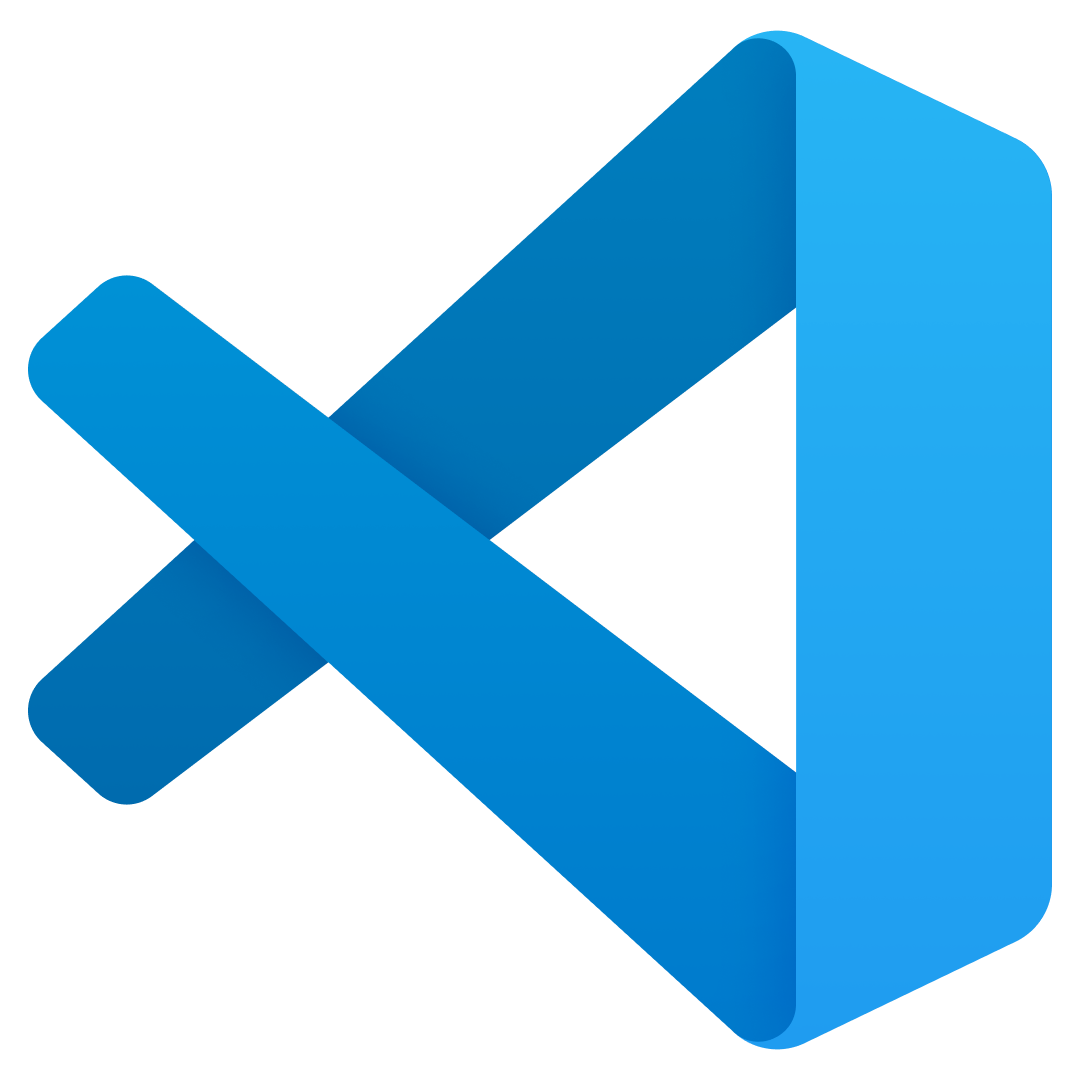
\includegraphics[width=0.20\textwidth]{vscode.png}
	\caption{Visual Studio Code Logo~\cite{vscode2024}}
	\label{fig:vscode_logo}
\end{figure}

\subsection{ROS 2 and Gazebo Simulation Environment}
An open-source middleware framework for creating robotic applications is called Robot Operating System~2 (ROS~2)~\cite{ros2jazzy2024}. It divides software into nodes, which are modular parts that interact with one another through action servers, services, and topics. The main basis for this project was ROS~2. The core of the system was ROS~2.

An open-source 3D robot simulator called Gazebo~\cite{gazebo2024} offers a physics-based environment for testing robotic systems prior to their implementation on actual hardware. To verify the navigation algorithms in a secure virtual setting, it was integrated with ROS~2. Based on the TurtleBot3 platform~\cite{turtlebot3doc}, the robot model had wheel encoders, a depth camera, and a simulated LiDAR. In order to test path planning, obstacle avoidance, and multi-waypoint delivery missions, custom indoor settings featuring walls, hallways, and obstacles were constructed. This eliminated the requirement to run unverified code on real hardware during development.

\begin{figure}[h]
	\centering
	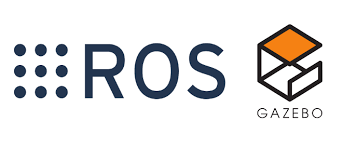
\includegraphics[width=0.3\textwidth]{ros.png}
	\caption{ROS~2 Jazzy Jalisco Logo~\cite{ros2jazzy2024}}
	\label{fig:ros2_logo}
\end{figure}

\subsection{Google Colaboratory}

A cloud platform called Google Colaboratory (Colab)~\cite{colab2024} offers a Jupyter notebook platform that enables users to develop and execute Python code in a web browser without requiring a local configuration. It provides unrestricted access to the GPU's processing capabilities, making it especially suitable for algorithm development and data analysis endeavors.

\begin{figure}[h]
	\centering
	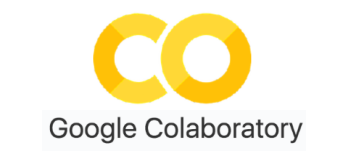
\includegraphics[width=0.5\textwidth]{colab.png}
	\caption{Google Colaboratory Logo~\cite{colab2024}}
	\label{fig:colab_logo}
\end{figure}

\subsection{GitHub}
GitHub~\cite{github2024} is an online platform that uses Git version control to store and manage source-code repositories.
It was used during the research in controlling the code, documenting changes and supporting interaction between members of a project. Each team member worked on separate branches, and then could combine changes through pull requests once they had been reviewed. GitHub also served as a reliable cloud backup protecting the project from data loss.
\begin{figure}[H]
	\centering
	
\includegraphics[width=0.4\textwidth]{github.png}
	\caption{GitHub Logo~\cite{github2024}}
	\label{fig:github_logo}
\end{figure}

\subsection{Flutter}

Flutter~\cite{flutter2024} is an open-source framework that Google created to create cross-platform mobile apps in the Dart programming language. It was applied in this project to create the mobile application frontend enabling the customers to make the delivery request, see the real-time location of the robot, and get the status messages. The hot reload support in Flutter allowed the development and testing of the UI quickly, and the cross-platform nature of this environment was useful in ensuring that the application is compatible with both the Android and iOS platforms without needing to maintain two separate codebases.

\begin{figure}[h!]
	\centering
	
\includegraphics[width=0.3\textwidth]{flutterjpg.jpg}
	\caption{Flutter Framework Logo~\cite{flutter2024}}
	\label{fig:flutter_logo}
\end{figure}

\subsection{Flask}

Flask~\cite{flask2024} is a lightweight Python framework that is employed in the development of web applications. It was used in this project to build up the back-end server which is responsible in dealing with the communication between the web application and the autonomous robot. The Flask server receives delivery requests using the mobile application, writes the information into the database, and dispatches the navigation instructions to the ROS 2 system.
\begin{figure}[H]
	\centering
	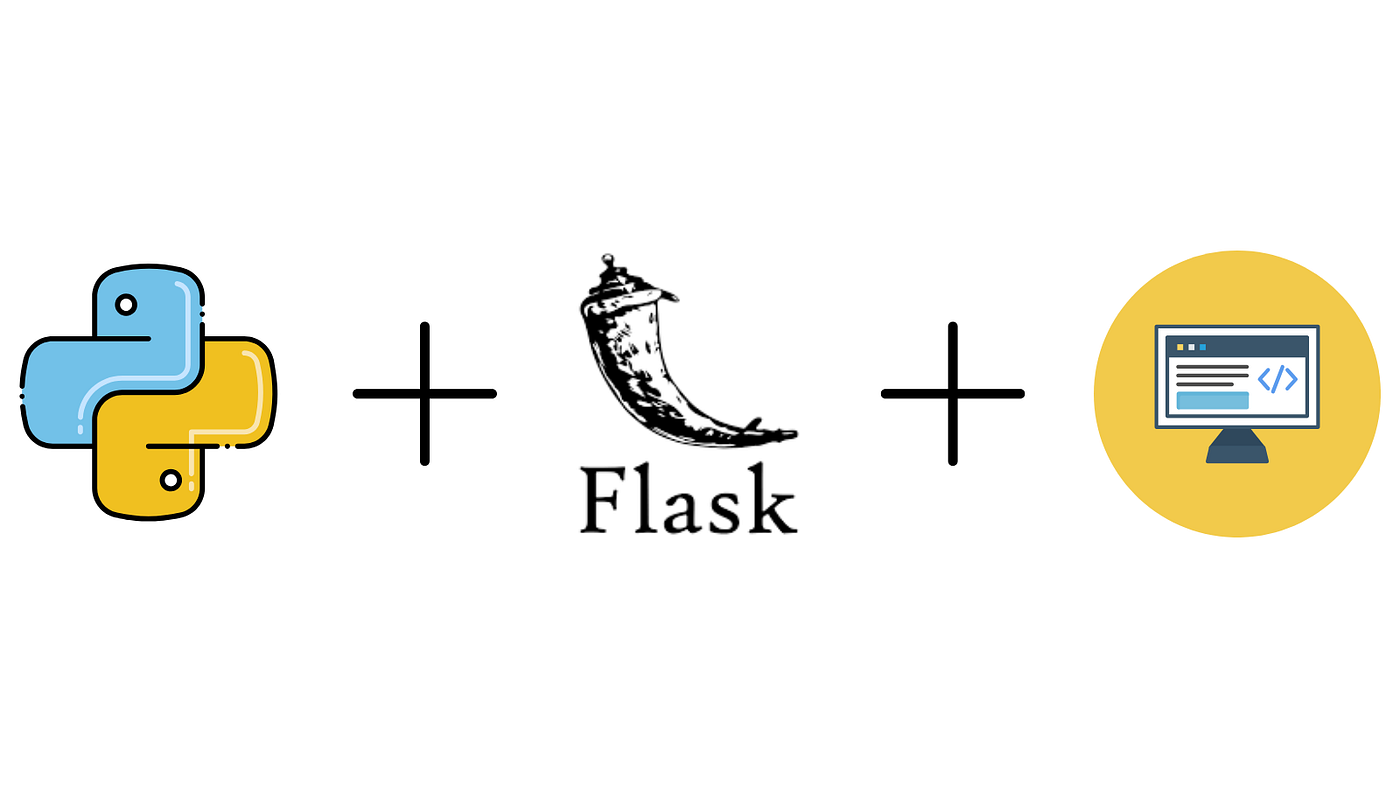
\includegraphics[width=0.5\textwidth]{flask.png}
	\caption{Python Flask Backend Architecture~\cite{flask2024}}
	\label{fig:flask_logo}
\end{figure}

\subsection{Overleaf}
Overleaf~\cite{overleaf2024} is an online collaborative LaTeX editor used for writing and formatting academic documents. It was utilized in this project to create the final report in compliance with Capital University of Science and Technology's (CUST) formatting specifications. A professionally designed paper with consistent headings, captions, equations, and IEEE-style citations was created by using LaTeX through Overleaf.

\begin{figure}[h]
	\centering
	
\includegraphics[width=0.3\textwidth]{overleaf.png}
	\caption{Overleaf Logo~\cite{overleaf2024}}
	\label{fig:overleaf_logo}
\end{figure}

\section{Summary}
The software tools utilized for the project were described in this chapter. Visual Studio Code was the primary IDE for all coding operations, and Oracle VirtualBox housed the Ubuntu development environment. Gazebo offered a physics-based simulation platform for testing navigation algorithms prior to hardware deployment, while ROS~2 Jazzy served as the fundamental robotics framework. Overleaf facilitated expert report creation, GitHub preserved version control and teamwork, while Google Colab helped early algorithm prototyping and SLAM implementation. Together, they supported every stage of the project, from concept to final documentation, and each tool was chosen for a particular function.